\section{High precision tracking detector for the ILC muon system}
Most recent update: 2018-06-04 \\
Contact person: Dmitri Denisov (denisovd@fnal.gov), Strahinja Lukić (slukic@vinca.rs)

\subsection{High-precision muon tracking with scintillators}

In a muon system with scintillator strips, the muon track is reconstructed using observables such as the position of the strip hit by a passing muon and the signal time difference $\Delta t$ between the ends of the strip to measure position along the strip. If a muon system has strip orientations alternating by $90^{\circ}$ in neighboring layers, the muon track can be reconstructed using only the positions of the strips that fired. In this case, the measurement of the position along each strip using $\Delta t$ serves to improve the precision of the track fit and to resolve ``ghosts'' arising at the intersections of strips hit by different particles. In the case when perpendicular orientation of strips is not feasible for access to the ends of the strips, time difference remains the only source of information about the longitudinal position.

To achieve sub-ns time resolution and a position resolution of several cm, the design of scintillator strips must employ the fastest available scintillator and WLS materials, as well as maximize the light yield per muon.

\subsection{Design and test of scintillator strips for high-precision muon tracking}

Excellent performance is observed when the Bicron\textsuperscript{\textcopyright} 404A fast clear scintillator strip with a $27 \times \SI{12}{mm^2}$ profile is used in a configuration with seven Bicron\textsuperscript{\textcopyright} BCF-92 WLS fibers of \SI{1.0}{mm} diameter attached to the narrower side of the strip using reflective adhesive tape (Figure~\ref{fig:design}) \cite{Denisov2016120}. For light isolation the strip is wrapped with one layer of the white Tyvek\textsuperscript{\textregistered} sheet and several layers of black Tedlar\textsuperscript{\textregistered} paper. Beyond the end of the strip, the ends of the fibers are bundled together in a tight hexagonal shape for optimal concentration of light on the surface of the SiPM photodetector. The strips are readout using Hamamatsu S13360-3050CS SiPMs operated in the ``high-gain'' mode, with high overvoltage resulting in a high photon detection efficiency.

\begin{figure}
  \centering
  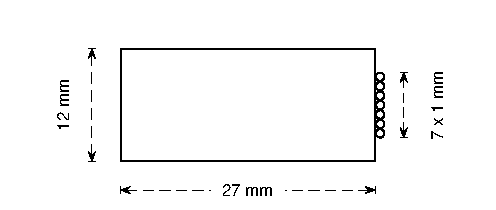
\includegraphics[width=.6\textwidth]{MuonDetector/Scintillator/bicron}
  \caption{\label{fig:design} Design of scintillator strip with WLS fibers
  for high-precision muon tracking.}
\end{figure}

This strip design was recently tested using the muon beam at the Fermilab Test Beam Facility (FTBF). Three plastic scintillator counters were aligned with the beam and used as the trigger for the passage of the muon (Figure~\ref{fig:setup}). The width of the counters \textsf{S1} and \textsf{S2} was \SI{2.5}{cm} in order to select muons in a narrow region to study position resolution. The average time of \textsf{S1} and \textsf{S2} was used as the time reference for the muon passage. Strips with \SI{1}{m} length were tested.

\begin{figure}[h!]
  \centering
  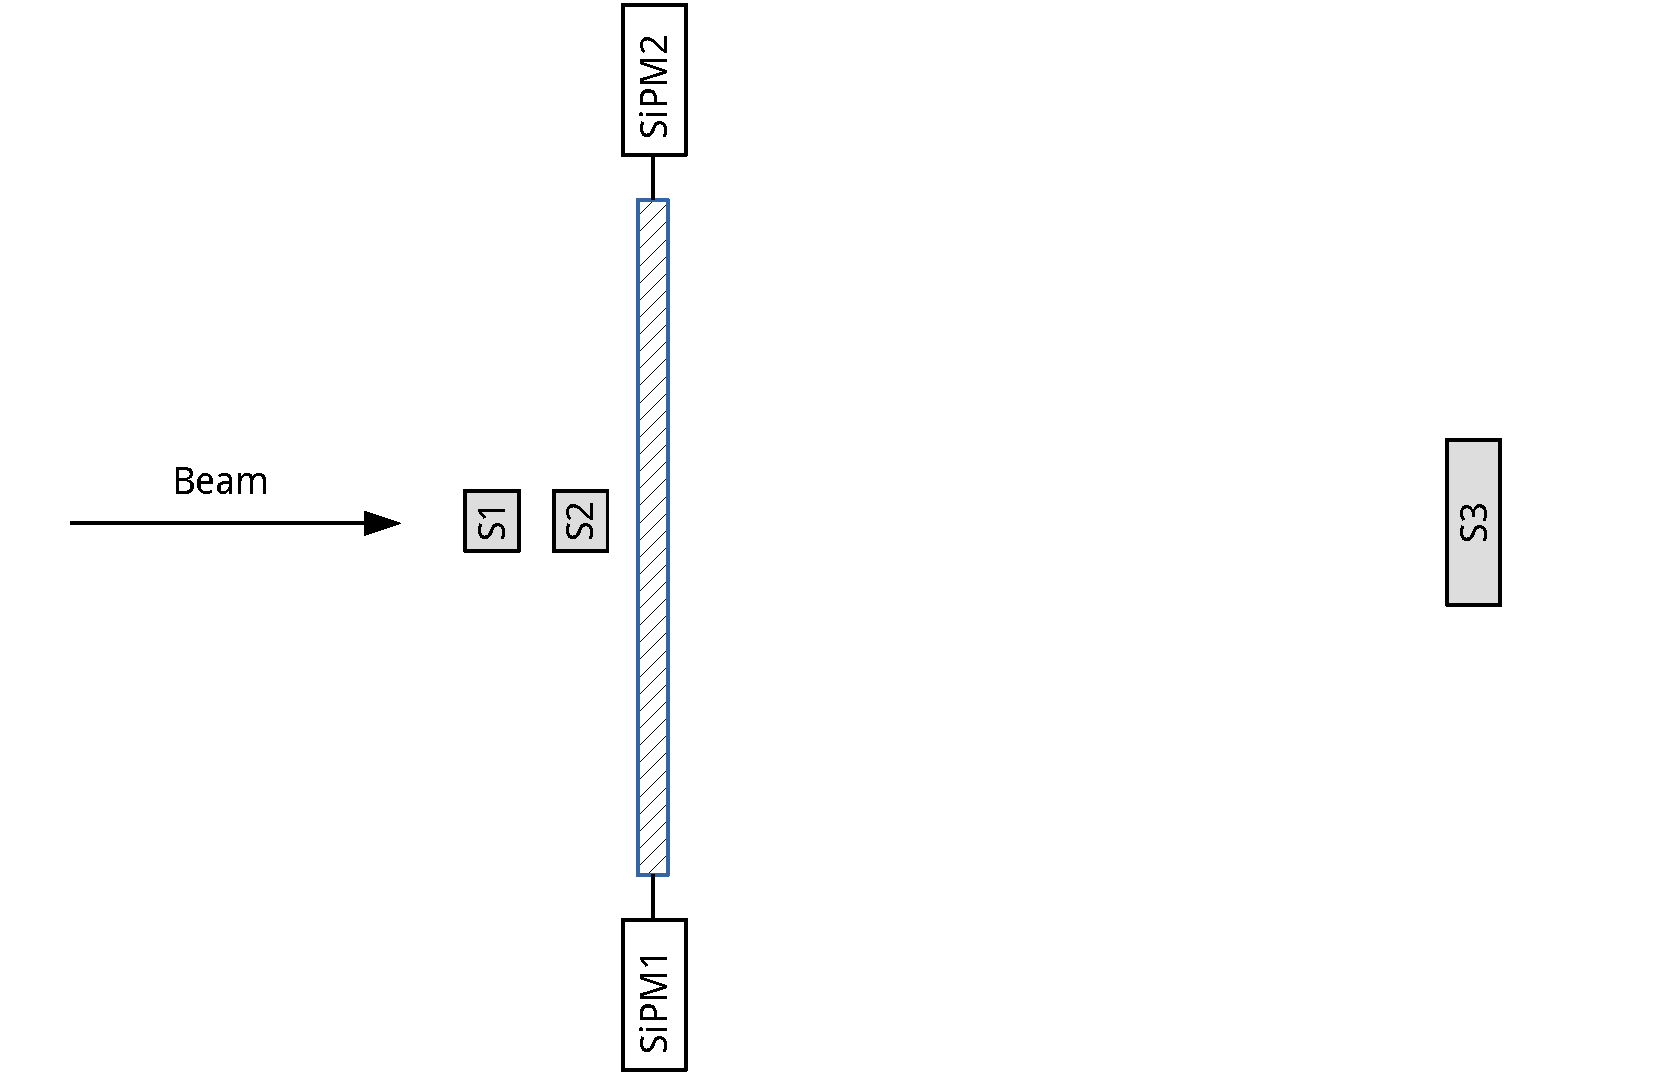
\includegraphics[width=.9\textwidth]{MuonDetector/Scintillator/setup}
  \caption{\label{fig:setup} Test setup for time and position resolution of scintillator strips for the muon system.}
\end{figure}


\subsection{Performance of the tested strips for the muon system}

The average number of photoelectrons per muon as a function of the longitudinal position is shown for both sides of the strip in Figure~\ref{fig:nphot}. Light attenuation along the strip is clearly seen.

\begin{figure}[h!]
\centering
   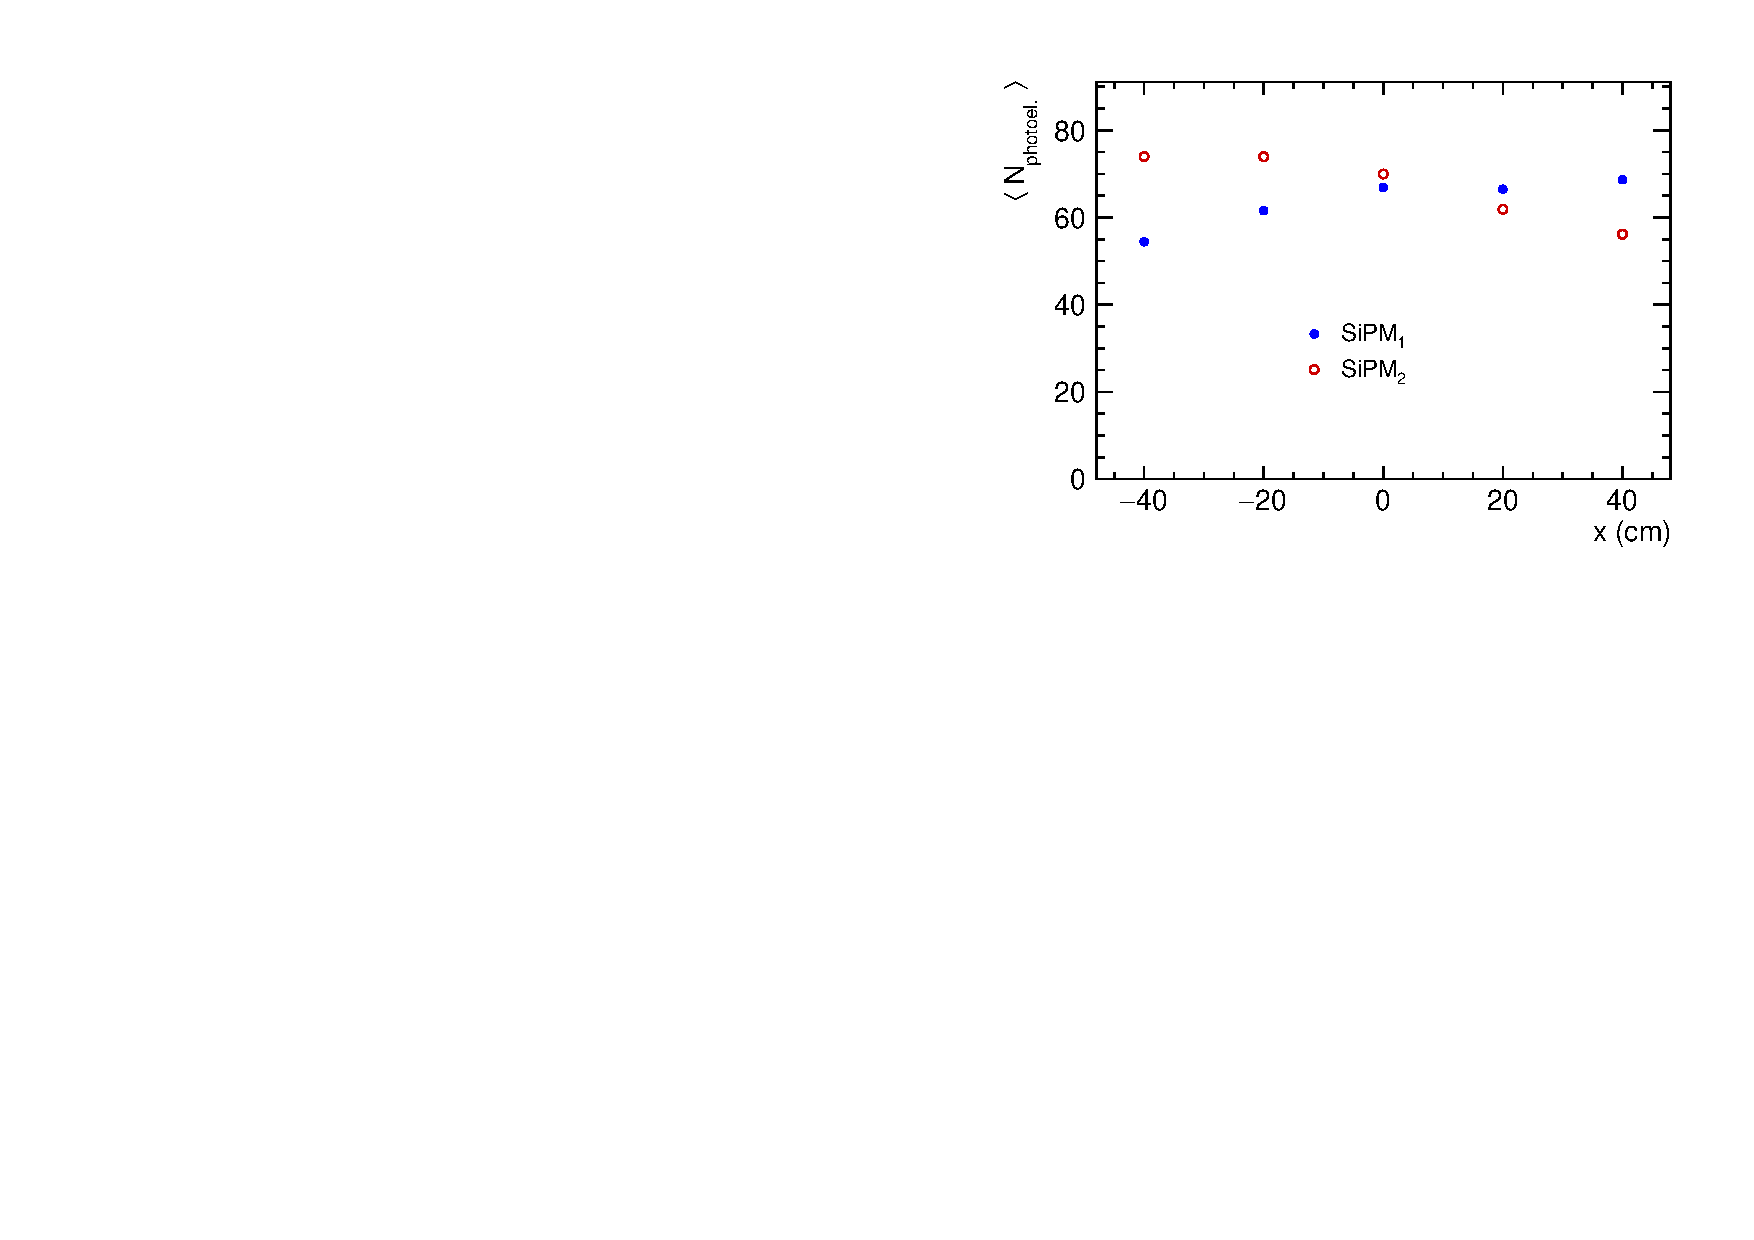
\includegraphics[width=.6\textwidth]{MuonDetector/Scintillator/nphot}
   \caption{\label{fig:nphot} Average number of photoelectrons per muon detected at the two ends of a scintillator strip as a function of the longitudinal position.}
\end{figure}

The relatively high number of photoelectrons per muon for this type of device results in excellent resolution of the muon time, calculated as the average time between the two ends. Similarly excellent resolution is obtained for the time difference between the two ends, the key observable for longitudinal position determination (Figure~\ref{fig:sigma-tdt}).

\begin{figure}[h!]
\centering
   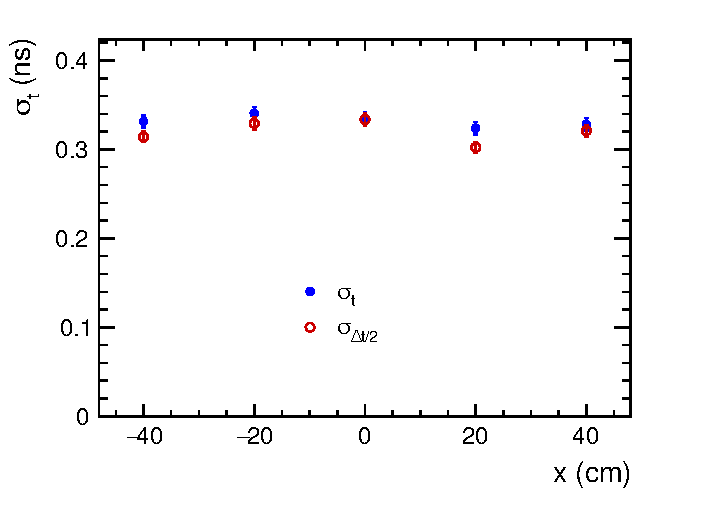
\includegraphics[width=.6\textwidth]{MuonDetector/Scintillator/sigma-tdt}
   \caption{\label{fig:sigma-tdt} Time resolution of the strip and resolution of the $\Delta t/2$ observable for longitudinal position determination, shown as a function of the longitudinal position.}
\end{figure}

Taking into account the measured signal propagation speed along the strips, \mbox{$v=\SI{16.9}{cm/ns}$} and the resolution $\sigma_{\Delta t/2} = \SI{0.33}{ns}$, the resulting resolution of the longitudinal position is $\sigma_x = \SI{5.4}{cm}$.

\subsection{References}
\fullcite{Denisov201754}

\subsection{Future plans}

In future muon systems, strip lengths of \SI{2}{m} or more are envisioned. Light attenuation in long strips will inevitably lead to worsening of the time and position resolution. Light attenuation length for WLS fibers used in the studies presented here is over \SI{3.5}{m}. Thus it is expected that the worsening of the time and position resolution will be small. This will be tested in the test beam using longer strips.
